\documentclass{article}

\usepackage{amsmath}
\usepackage{amssymb}
\usepackage{amsfonts}
\usepackage{mathtools}

\usepackage{graphicx}

\usepackage[thmmarks, amsmath]{ntheorem}

\usepackage{diffcoeff}
\usepackage{cancel}

\usepackage{enumitem}

\setlist{label=\alph*)}

\title{Differential Geometry Homework 3}
\author{Duarte Maia}
\date{}

\theorembodyfont{\upshape}
\theoremseparator{.}
\newtheorem{ex}{Exercise}

\theoremstyle{nonumberplain}
\theoremheaderfont{\itshape}
\theorembodyfont{\upshape}
\theoremseparator{:}
\theoremsymbol{\ensuremath{\blacksquare}}
\newtheorem{sol}{Solution}

\newcommand{\R}{\mathbb{R}}
\newcommand{\C}{\mathbb{C}}
\newcommand{\Z}{\mathbb{Z}}

\newcommand{\PP}{\mathbb{P}}
\newcommand{\FF}{\mathcal{F}}

\newcommand{\I}{\mathrm{i}}
\newcommand{\e}{\mathrm{e}}


\DeclareMathOperator{\inte}{int}
\DeclareMathOperator{\codim}{codim}
\newcommand{\grad}{\nabla}

\DeclarePairedDelimiter{\norm}{\lvert}{\rvert}

\begin{document}
\maketitle

\begin{ex}
Give an example of a one-dimensional distribution which is not globally generated by a vector field.
\end{ex}

\begin{sol}
Consider the (open) Möbius strip, given by a square with the left and right side identified with opposite orientations. Then, the `vertical distribution' is not globally generated. To show this, we may cover the Möbius strip into two rectangular charts such as in the following figure:

\begin{center}
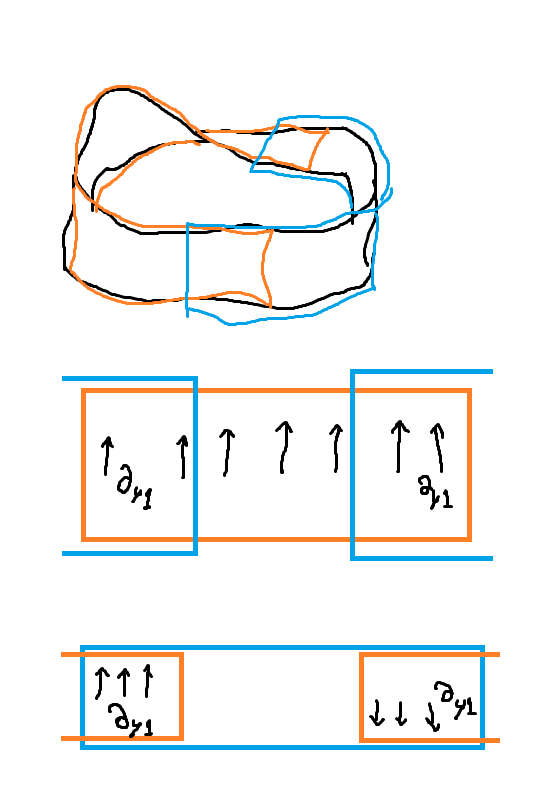
\includegraphics[width=.7\linewidth]{mobcharts}
\end{center}

We use $\partial_{y1}$ to represent the coordinate $y$ vector in the orange chart, and $\partial_{y2}$ to represent the coordinate $y$ vector in the blue chart. The important thing to note is that the charts intersect at two rectangles. In one of them, $\partial_{y1} = \partial_{y2}$, while in the other $\partial_{y1} = - \partial_{y2}$.

Now, the distribution at hand is locally generated by these coordinate $y$ vectors. However, it cannot be globally generated. Indeed, if $X$ were a vector field that globally generated the vertical distribution, then over the orange chart it would have to be of the form $f \partial_{y1}$, where $f$ is never null, and therefore could never change sign because the orange chart is connected. A similar argument shows that over the blue chart $X$ would be of the form $g \partial_{y2}$, where $g$ never changes sign. But this yields a contradiction, because over the intersection $X$ must be of the form
\[f \partial_{y1} = g \partial_{y2},\]
where $f$ and $g$ never change signs. If we look at the section where $\partial_{y1} = \partial_{y2}$ we conclude that the signs of $f$ and $g$ must be the same, but if we look at the section where $\partial_{y1} = - \partial_{y2}$ their signs must be opposite. This contradiction proves that the vector field $X$ cannot exist.
\end{sol}

\begin{ex}
Let $G$, $H$ be connected Lie groups and $\phi \colon G \to H$ a smooth homomorphism. Suppose that $(\dl \phi)_e$ is an isomorphism. Show that $\phi$ is a covering map.
\end{ex}

\begin{sol}
Since $(\dl \phi)_e$ is an isomorphism, there exists a neighborhood of the identity, say $U \subseteq G$, such that $\phi$ is a diffeomorphism from $U$ to $\phi(U)$.
\end{sol}

\begin{ex}
\end{ex}

\begin{sol}
\end{sol}

\begin{ex}
\end{ex}

\begin{sol}
\end{sol}

\begin{ex}
\end{ex}

\begin{sol}
\end{sol}

\end{document}